\PassOptionsToPackage{unicode=true}{hyperref} % options for packages loaded elsewhere
\PassOptionsToPackage{hyphens}{url}
%
\documentclass[]{article}
\usepackage{lmodern}
\usepackage{amssymb,amsmath}
\usepackage{ifxetex,ifluatex}
\usepackage{fixltx2e} % provides \textsubscript
\ifnum 0\ifxetex 1\fi\ifluatex 1\fi=0 % if pdftex
  \usepackage[T1]{fontenc}
  \usepackage[utf8]{inputenc}
  \usepackage{textcomp} % provides euro and other symbols
\else % if luatex or xelatex
  \usepackage{unicode-math}
  \defaultfontfeatures{Ligatures=TeX,Scale=MatchLowercase}
\fi
% use upquote if available, for straight quotes in verbatim environments
\IfFileExists{upquote.sty}{\usepackage{upquote}}{}
% use microtype if available
\IfFileExists{microtype.sty}{%
\usepackage[]{microtype}
\UseMicrotypeSet[protrusion]{basicmath} % disable protrusion for tt fonts
}{}
\IfFileExists{parskip.sty}{%
\usepackage{parskip}
}{% else
\setlength{\parindent}{0pt}
\setlength{\parskip}{6pt plus 2pt minus 1pt}
}
\usepackage{hyperref}
\hypersetup{
            pdftitle={Lecture 5},
            pdfauthor={Jung-Jin Lee},
            pdfborder={0 0 0},
            breaklinks=true}
\urlstyle{same}  % don't use monospace font for urls
\usepackage[margin=1in]{geometry}
\usepackage{color}
\usepackage{fancyvrb}
\newcommand{\VerbBar}{|}
\newcommand{\VERB}{\Verb[commandchars=\\\{\}]}
\DefineVerbatimEnvironment{Highlighting}{Verbatim}{commandchars=\\\{\}}
% Add ',fontsize=\small' for more characters per line
\usepackage{framed}
\definecolor{shadecolor}{RGB}{248,248,248}
\newenvironment{Shaded}{\begin{snugshade}}{\end{snugshade}}
\newcommand{\AlertTok}[1]{\textcolor[rgb]{0.94,0.16,0.16}{#1}}
\newcommand{\AnnotationTok}[1]{\textcolor[rgb]{0.56,0.35,0.01}{\textbf{\textit{#1}}}}
\newcommand{\AttributeTok}[1]{\textcolor[rgb]{0.77,0.63,0.00}{#1}}
\newcommand{\BaseNTok}[1]{\textcolor[rgb]{0.00,0.00,0.81}{#1}}
\newcommand{\BuiltInTok}[1]{#1}
\newcommand{\CharTok}[1]{\textcolor[rgb]{0.31,0.60,0.02}{#1}}
\newcommand{\CommentTok}[1]{\textcolor[rgb]{0.56,0.35,0.01}{\textit{#1}}}
\newcommand{\CommentVarTok}[1]{\textcolor[rgb]{0.56,0.35,0.01}{\textbf{\textit{#1}}}}
\newcommand{\ConstantTok}[1]{\textcolor[rgb]{0.00,0.00,0.00}{#1}}
\newcommand{\ControlFlowTok}[1]{\textcolor[rgb]{0.13,0.29,0.53}{\textbf{#1}}}
\newcommand{\DataTypeTok}[1]{\textcolor[rgb]{0.13,0.29,0.53}{#1}}
\newcommand{\DecValTok}[1]{\textcolor[rgb]{0.00,0.00,0.81}{#1}}
\newcommand{\DocumentationTok}[1]{\textcolor[rgb]{0.56,0.35,0.01}{\textbf{\textit{#1}}}}
\newcommand{\ErrorTok}[1]{\textcolor[rgb]{0.64,0.00,0.00}{\textbf{#1}}}
\newcommand{\ExtensionTok}[1]{#1}
\newcommand{\FloatTok}[1]{\textcolor[rgb]{0.00,0.00,0.81}{#1}}
\newcommand{\FunctionTok}[1]{\textcolor[rgb]{0.00,0.00,0.00}{#1}}
\newcommand{\ImportTok}[1]{#1}
\newcommand{\InformationTok}[1]{\textcolor[rgb]{0.56,0.35,0.01}{\textbf{\textit{#1}}}}
\newcommand{\KeywordTok}[1]{\textcolor[rgb]{0.13,0.29,0.53}{\textbf{#1}}}
\newcommand{\NormalTok}[1]{#1}
\newcommand{\OperatorTok}[1]{\textcolor[rgb]{0.81,0.36,0.00}{\textbf{#1}}}
\newcommand{\OtherTok}[1]{\textcolor[rgb]{0.56,0.35,0.01}{#1}}
\newcommand{\PreprocessorTok}[1]{\textcolor[rgb]{0.56,0.35,0.01}{\textit{#1}}}
\newcommand{\RegionMarkerTok}[1]{#1}
\newcommand{\SpecialCharTok}[1]{\textcolor[rgb]{0.00,0.00,0.00}{#1}}
\newcommand{\SpecialStringTok}[1]{\textcolor[rgb]{0.31,0.60,0.02}{#1}}
\newcommand{\StringTok}[1]{\textcolor[rgb]{0.31,0.60,0.02}{#1}}
\newcommand{\VariableTok}[1]{\textcolor[rgb]{0.00,0.00,0.00}{#1}}
\newcommand{\VerbatimStringTok}[1]{\textcolor[rgb]{0.31,0.60,0.02}{#1}}
\newcommand{\WarningTok}[1]{\textcolor[rgb]{0.56,0.35,0.01}{\textbf{\textit{#1}}}}
\usepackage{graphicx,grffile}
\makeatletter
\def\maxwidth{\ifdim\Gin@nat@width>\linewidth\linewidth\else\Gin@nat@width\fi}
\def\maxheight{\ifdim\Gin@nat@height>\textheight\textheight\else\Gin@nat@height\fi}
\makeatother
% Scale images if necessary, so that they will not overflow the page
% margins by default, and it is still possible to overwrite the defaults
% using explicit options in \includegraphics[width, height, ...]{}
\setkeys{Gin}{width=\maxwidth,height=\maxheight,keepaspectratio}
\setlength{\emergencystretch}{3em}  % prevent overfull lines
\providecommand{\tightlist}{%
  \setlength{\itemsep}{0pt}\setlength{\parskip}{0pt}}
\setcounter{secnumdepth}{0}
% Redefines (sub)paragraphs to behave more like sections
\ifx\paragraph\undefined\else
\let\oldparagraph\paragraph
\renewcommand{\paragraph}[1]{\oldparagraph{#1}\mbox{}}
\fi
\ifx\subparagraph\undefined\else
\let\oldsubparagraph\subparagraph
\renewcommand{\subparagraph}[1]{\oldsubparagraph{#1}\mbox{}}
\fi

% set default figure placement to htbp
\makeatletter
\def\fps@figure{htbp}
\makeatother


\title{Lecture 5}
\author{Jung-Jin Lee}
\date{2/4/2020}

\begin{document}
\maketitle

\begin{Shaded}
\begin{Highlighting}[]
\NormalTok{ht <-}\StringTok{ }\KeywordTok{read.table}\NormalTok{(}\DataTypeTok{file =} \StringTok{"heights.txt"}\NormalTok{, }\DataTypeTok{header =}\NormalTok{ T, }\DataTypeTok{sep =} \StringTok{" "}\NormalTok{)}
\KeywordTok{ggplot}\NormalTok{(ht, }\KeywordTok{aes}\NormalTok{(Mheight)) }\OperatorTok{+}\StringTok{ }
\StringTok{  }\KeywordTok{geom_histogram}\NormalTok{()}
\end{Highlighting}
\end{Shaded}

\begin{verbatim}
## `stat_bin()` using `bins = 30`. Pick better value with `binwidth`.
\end{verbatim}

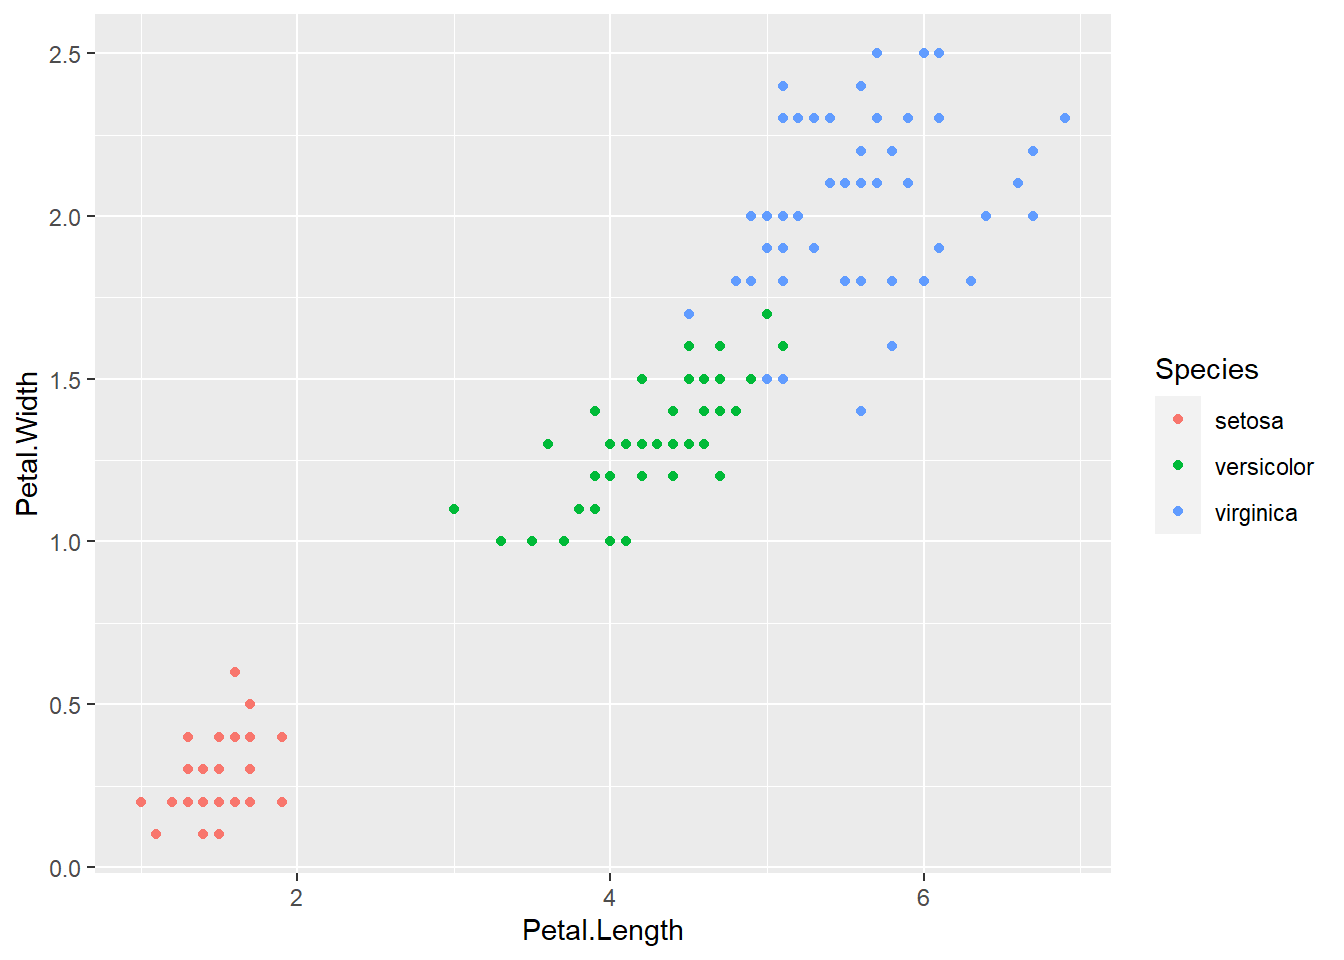
\includegraphics{lecture5_files/figure-latex/unnamed-chunk-1-1.pdf}

\begin{Shaded}
\begin{Highlighting}[]
\KeywordTok{mean}\NormalTok{(ht}\OperatorTok{$}\NormalTok{Mheight)}
\end{Highlighting}
\end{Shaded}

\begin{verbatim}
## [1] 62.4528
\end{verbatim}

\begin{Shaded}
\begin{Highlighting}[]
\KeywordTok{sd}\NormalTok{(ht}\OperatorTok{$}\NormalTok{Mheight)}
\end{Highlighting}
\end{Shaded}

\begin{verbatim}
## [1] 2.355103
\end{verbatim}

\begin{Shaded}
\begin{Highlighting}[]
\KeywordTok{t.test}\NormalTok{(ht}\OperatorTok{$}\NormalTok{Mheight)}
\end{Highlighting}
\end{Shaded}

\begin{verbatim}
## 
##  One Sample t-test
## 
## data:  ht$Mheight
## t = 983.32, df = 1374, p-value < 2.2e-16
## alternative hypothesis: true mean is not equal to 0
## 95 percent confidence interval:
##  62.32821 62.57739
## sample estimates:
## mean of x 
##   62.4528
\end{verbatim}

\begin{Shaded}
\begin{Highlighting}[]
\NormalTok{mu <-}\StringTok{ }\FloatTok{62.2} \CommentTok{# null hypothesis}
\NormalTok{x <-}\StringTok{ }\NormalTok{ht}\OperatorTok{$}\NormalTok{Mheight}
\NormalTok{xbar <-}\StringTok{ }\KeywordTok{mean}\NormalTok{(x); S <-}\StringTok{ }\KeywordTok{sd}\NormalTok{(x); n <-}\StringTok{ }\KeywordTok{length}\NormalTok{(x)}
\NormalTok{t <-}\StringTok{ }\NormalTok{(xbar }\OperatorTok{-}\StringTok{ }\NormalTok{mu) }\OperatorTok{/}\StringTok{ }\NormalTok{(S}\OperatorTok{/}\KeywordTok{sqrt}\NormalTok{(n)) }
\KeywordTok{print}\NormalTok{(xbar)}
\end{Highlighting}
\end{Shaded}

\begin{verbatim}
## [1] 62.4528
\end{verbatim}

\begin{Shaded}
\begin{Highlighting}[]
\KeywordTok{print}\NormalTok{(S)}
\end{Highlighting}
\end{Shaded}

\begin{verbatim}
## [1] 2.355103
\end{verbatim}

\begin{Shaded}
\begin{Highlighting}[]
\NormalTok{n}
\end{Highlighting}
\end{Shaded}

\begin{verbatim}
## [1] 1375
\end{verbatim}

\begin{Shaded}
\begin{Highlighting}[]
\NormalTok{t}
\end{Highlighting}
\end{Shaded}

\begin{verbatim}
## [1] 3.980324
\end{verbatim}

\begin{Shaded}
\begin{Highlighting}[]
\NormalTok{p.value <-}\StringTok{ }\DecValTok{2}\OperatorTok{*}\NormalTok{(}\DecValTok{1} \OperatorTok{-}\StringTok{ }\KeywordTok{pt}\NormalTok{(t, }\DataTypeTok{df =}\NormalTok{ n}\DecValTok{-1}\NormalTok{))}
\end{Highlighting}
\end{Shaded}

\begin{Shaded}
\begin{Highlighting}[]
\NormalTok{y <-}\StringTok{ }\NormalTok{ht}\OperatorTok{$}\NormalTok{Dheight}
\KeywordTok{t.test}\NormalTok{(y, }\DataTypeTok{mu =} \FloatTok{63.8}\NormalTok{)}
\end{Highlighting}
\end{Shaded}

\begin{verbatim}
## 
##  One Sample t-test
## 
## data:  y
## t = -0.69804, df = 1374, p-value = 0.4853
## alternative hypothesis: true mean is not equal to 63.8
## 95 percent confidence interval:
##  63.6135 63.8886
## sample estimates:
## mean of x 
##  63.75105
\end{verbatim}

\begin{Shaded}
\begin{Highlighting}[]
\KeywordTok{t.test}\NormalTok{(iris}\OperatorTok{$}\NormalTok{Sepal.Length, }\DataTypeTok{mu =} \FloatTok{5.1}\NormalTok{)}
\end{Highlighting}
\end{Shaded}

\begin{verbatim}
## 
##  One Sample t-test
## 
## data:  iris$Sepal.Length
## t = 10.994, df = 149, p-value < 2.2e-16
## alternative hypothesis: true mean is not equal to 5.1
## 95 percent confidence interval:
##  5.709732 5.976934
## sample estimates:
## mean of x 
##  5.843333
\end{verbatim}

\begin{Shaded}
\begin{Highlighting}[]
\NormalTok{crabs <-}\StringTok{ }\KeywordTok{read.table}\NormalTok{(}\StringTok{"crabs.tsv"}\NormalTok{, }\DataTypeTok{header =}\NormalTok{ T, }\DataTypeTok{sep =} \StringTok{"}\CharTok{\textbackslash{}t}\StringTok{"}\NormalTok{) }
\KeywordTok{dim}\NormalTok{(crabs)}
\end{Highlighting}
\end{Shaded}

\begin{verbatim}
## [1] 173   5
\end{verbatim}

\begin{Shaded}
\begin{Highlighting}[]
\CommentTok{# column names of crabs?}
\KeywordTok{names}\NormalTok{(crabs)}
\end{Highlighting}
\end{Shaded}

\begin{verbatim}
## [1] "color"  "spine"  "width"  "satell" "weight"
\end{verbatim}

\begin{Shaded}
\begin{Highlighting}[]
\NormalTok{crabs <-}\StringTok{ }\NormalTok{crabs }\OperatorTok
\StringTok{  }\KeywordTok{mutate}\NormalTok{(}\DataTypeTok{color =} \KeywordTok{factor}\NormalTok{(color)) }\OperatorTok
\StringTok{  }\KeywordTok{mutate}\NormalTok{(}\DataTypeTok{spine =} \KeywordTok{factor}\NormalTok{(spine)) }\OperatorTok
\StringTok{  }\KeywordTok{mutate}\NormalTok{(}\DataTypeTok{id =} \KeywordTok{paste0}\NormalTok{(}\StringTok{"obs"}\NormalTok{, }\DecValTok{1}\OperatorTok{:}\KeywordTok{nrow}\NormalTok{(crabs)))}
\end{Highlighting}
\end{Shaded}

\begin{Shaded}
\begin{Highlighting}[]
\NormalTok{crabs }\OperatorTok
\StringTok{  }\KeywordTok{ggplot}\NormalTok{(}\KeywordTok{aes}\NormalTok{(width)) }\OperatorTok{+}
\StringTok{  }\KeywordTok{geom_histogram}\NormalTok{(}\DataTypeTok{bins =} \DecValTok{10}\NormalTok{) }\OperatorTok{+}
\StringTok{  }\KeywordTok{facet_wrap}\NormalTok{(}\OperatorTok{~}\NormalTok{spine)}
\end{Highlighting}
\end{Shaded}

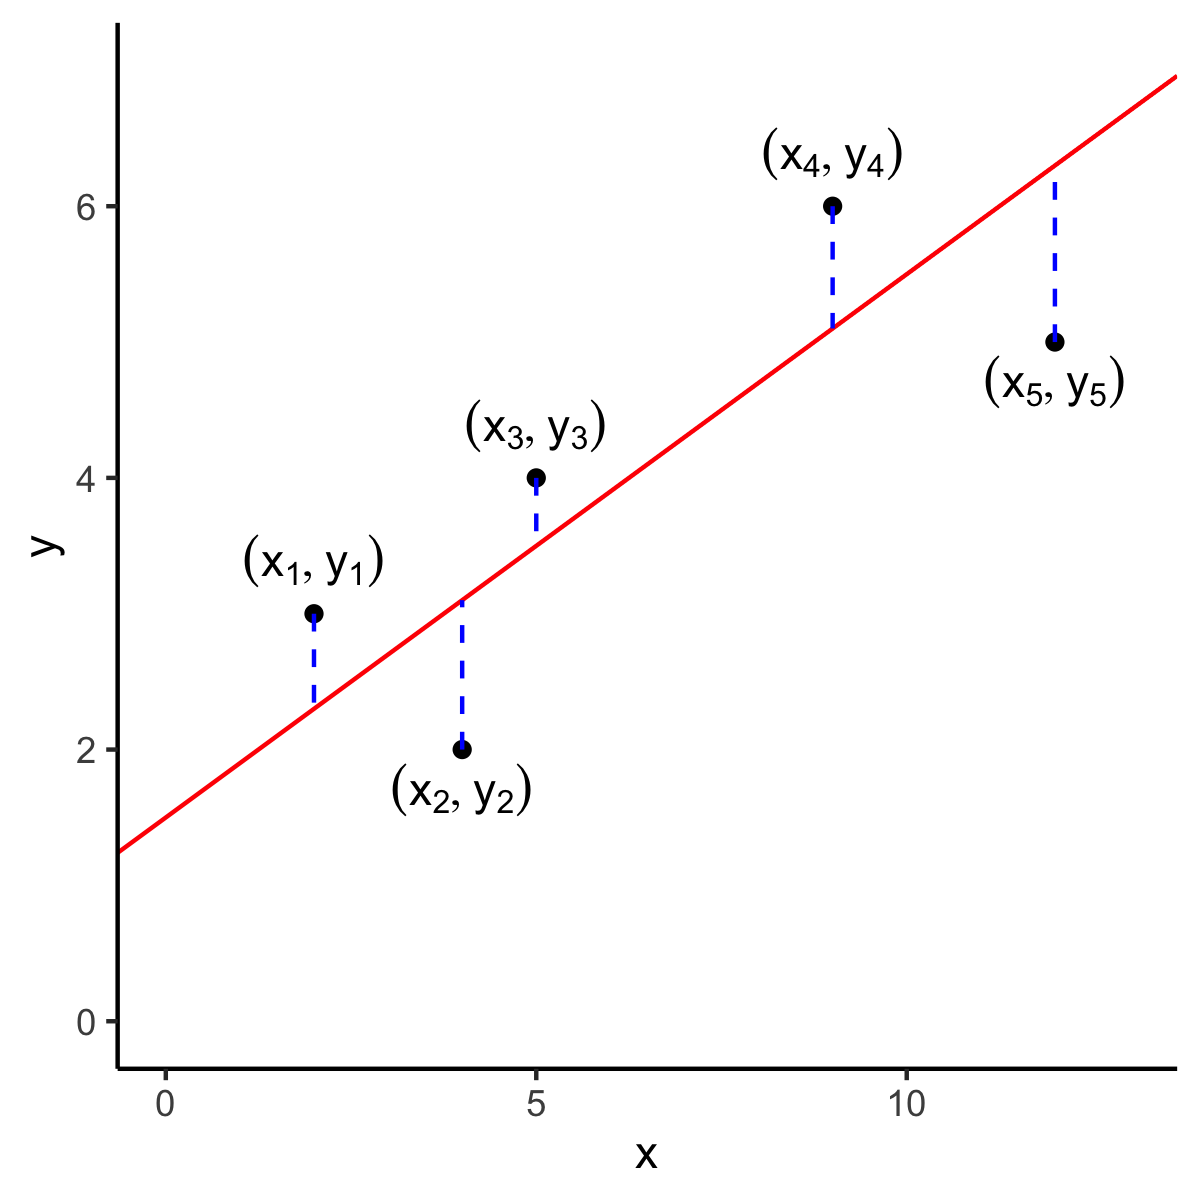
\includegraphics{lecture5_files/figure-latex/unnamed-chunk-6-1.pdf}

\begin{Shaded}
\begin{Highlighting}[]
\NormalTok{crabs }\OperatorTok
\StringTok{  }\KeywordTok{ggplot}\NormalTok{(}\KeywordTok{aes}\NormalTok{(color, weight)) }\OperatorTok{+}
\StringTok{  }\KeywordTok{geom_boxplot}\NormalTok{()}
\end{Highlighting}
\end{Shaded}

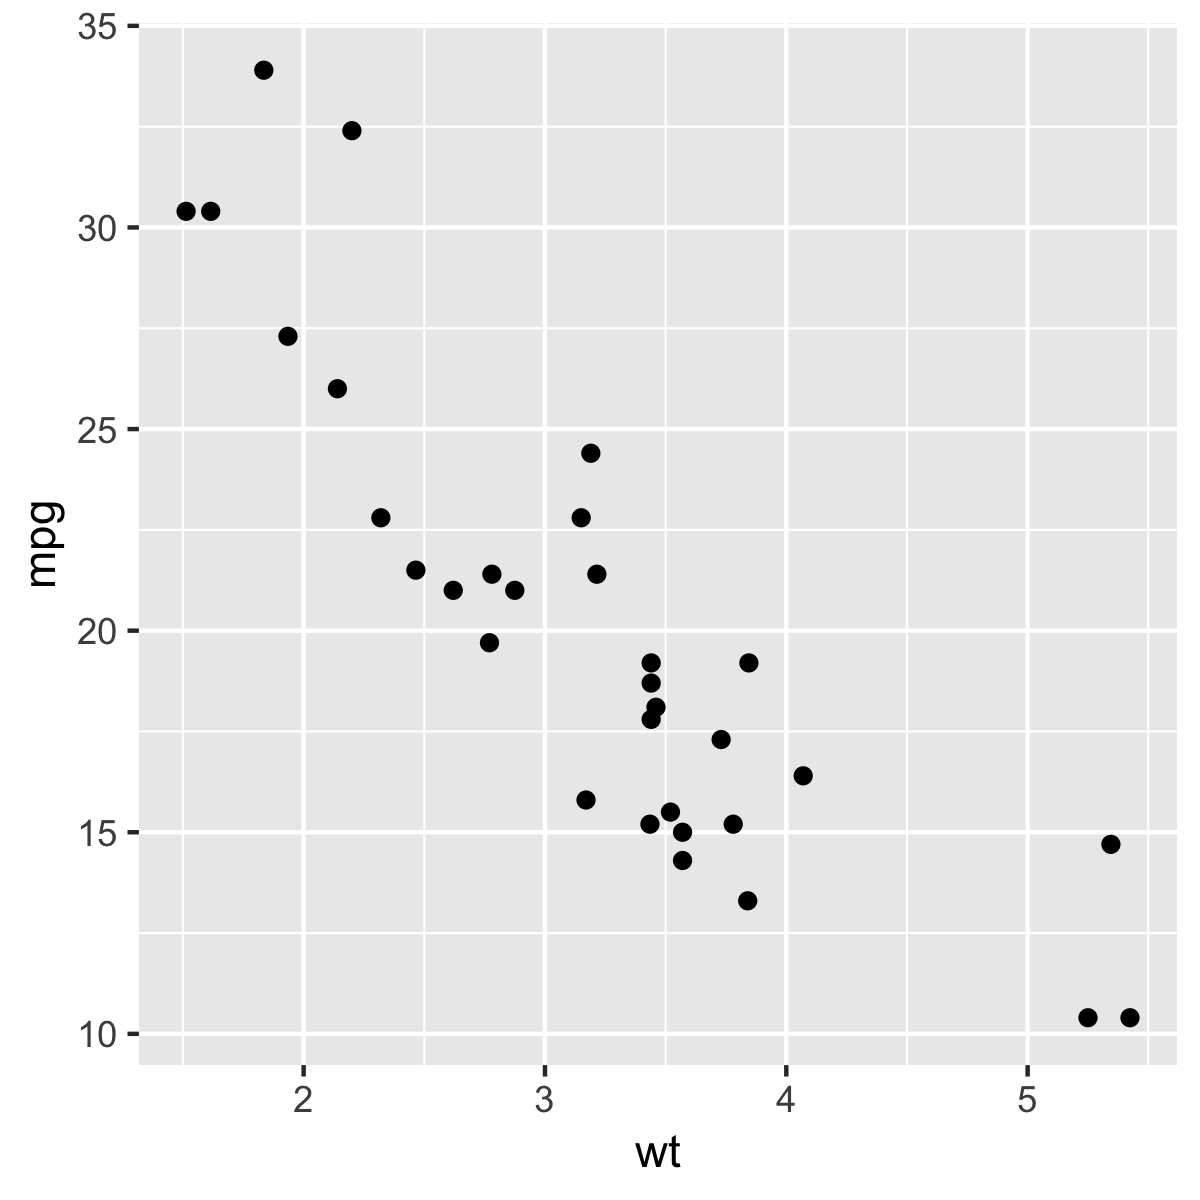
\includegraphics{lecture5_files/figure-latex/unnamed-chunk-7-1.pdf}

\begin{Shaded}
\begin{Highlighting}[]
\NormalTok{crabs }\OperatorTok
\StringTok{  }\KeywordTok{arrange}\NormalTok{(}\KeywordTok{desc}\NormalTok{(weight)) }\OperatorTok
\StringTok{  }\KeywordTok{head}\NormalTok{()}
\end{Highlighting}
\end{Shaded}

\begin{verbatim}
##   color spine width satell weight     id
## 1     3     1  33.5      7   5200 obs141
## 2     3     1  29.7      5   3850  obs91
## 3     3     1  31.7      4   3725 obs147
## 4     3     1  30.3      3   3600  obs50
## 5     4     2  29.8      4   3500 obs160
## 6     3     3  31.9      2   3325 obs115
\end{verbatim}

\begin{Shaded}
\begin{Highlighting}[]
\NormalTok{crabs }\OperatorTok
\StringTok{  }\KeywordTok{filter}\NormalTok{(color }\OperatorTok{==}\StringTok{ }\DecValTok{5}\NormalTok{) }\OperatorTok
\StringTok{  }\KeywordTok{arrange}\NormalTok{(}\KeywordTok{desc}\NormalTok{(weight)) }\OperatorTok
\StringTok{  }\KeywordTok{head}\NormalTok{()}
\end{Highlighting}
\end{Shaded}

\begin{verbatim}
##   color spine width satell weight     id
## 1     5     3  29.3     12   3225 obs117
## 2     5     3  27.5      0   2900  obs82
## 3     5     1  25.5      0   2750  obs88
## 4     5     3  27.0      0   2625 obs172
## 5     5     3  27.5      0   2600  obs29
## 6     5     3  26.7      0   2450  obs93
\end{verbatim}

\begin{Shaded}
\begin{Highlighting}[]
\CommentTok{#association between satell and weight}
\NormalTok{crabs }\OperatorTok
\StringTok{  }\KeywordTok{ggplot}\NormalTok{(}\KeywordTok{aes}\NormalTok{(weight, satell)) }\OperatorTok{+}
\StringTok{  }\KeywordTok{geom_point}\NormalTok{()}
\end{Highlighting}
\end{Shaded}

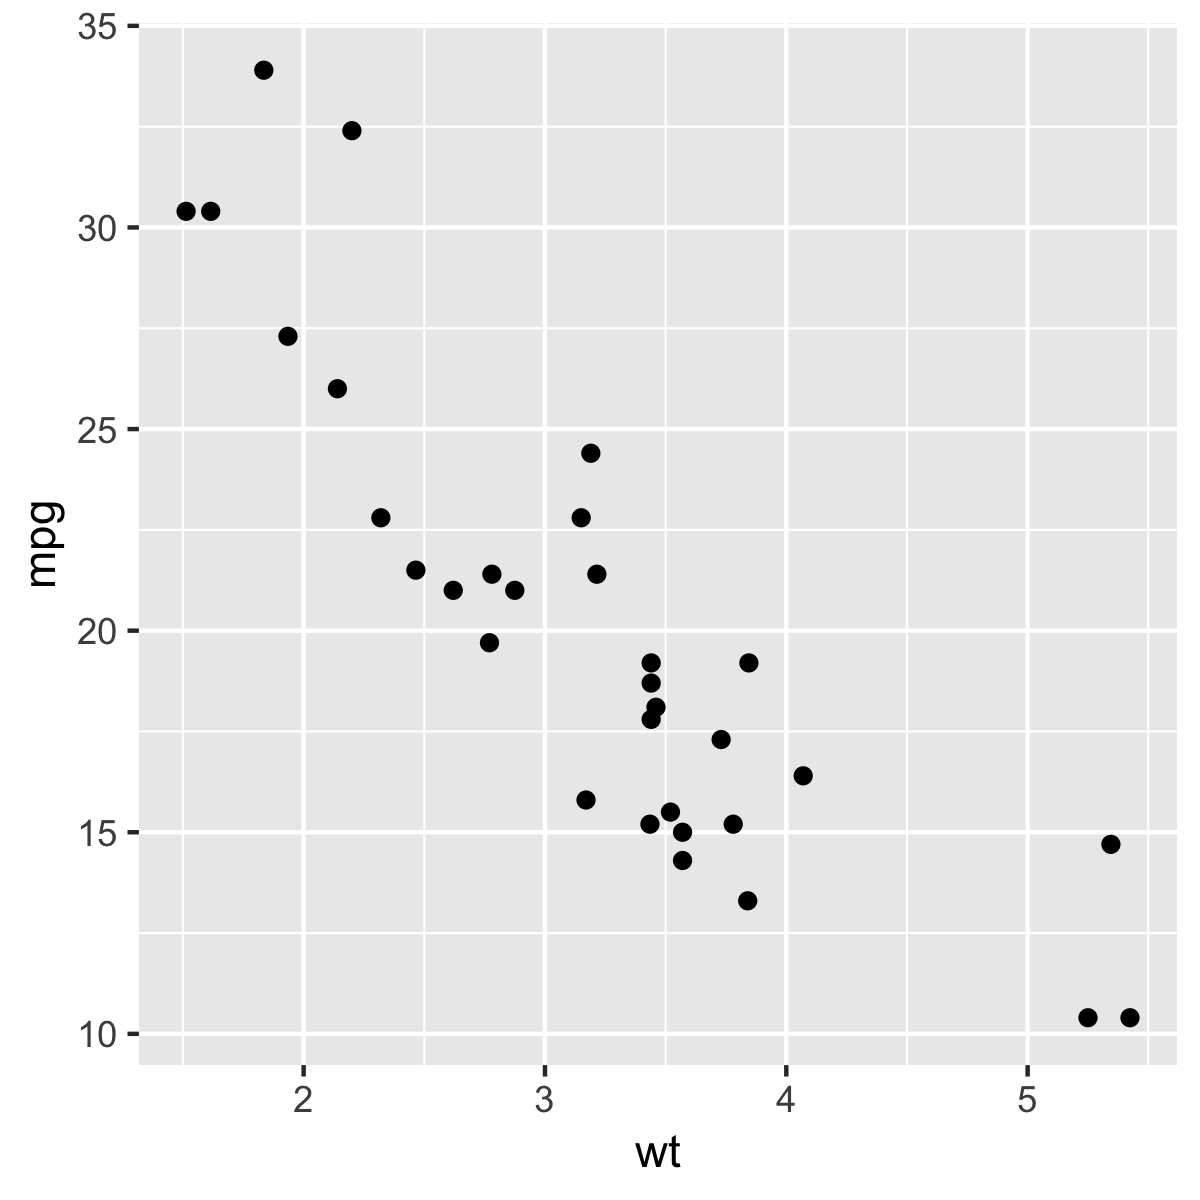
\includegraphics{lecture5_files/figure-latex/unnamed-chunk-10-1.pdf}

\begin{Shaded}
\begin{Highlighting}[]
\KeywordTok{t.test}\NormalTok{(crabs}\OperatorTok{$}\NormalTok{width, }\DataTypeTok{mu =} \DecValTok{26}\NormalTok{)}
\end{Highlighting}
\end{Shaded}

\begin{verbatim}
## 
##  One Sample t-test
## 
## data:  crabs$width
## t = 1.8637, df = 172, p-value = 0.06407
## alternative hypothesis: true mean is not equal to 26
## 95 percent confidence interval:
##  25.98234 26.61535
## sample estimates:
## mean of x 
##  26.29884
\end{verbatim}

\begin{Shaded}
\begin{Highlighting}[]
\KeywordTok{t.test}\NormalTok{(crabs}\OperatorTok{$}\NormalTok{weight, }\DataTypeTok{mu =} \DecValTok{2300}\NormalTok{)}
\end{Highlighting}
\end{Shaded}

\begin{verbatim}
## 
##  One Sample t-test
## 
## data:  crabs$weight
## t = 3.1272, df = 172, p-value = 0.002073
## alternative hypothesis: true mean is not equal to 2300
## 95 percent confidence interval:
##  2350.597 2523.784
## sample estimates:
## mean of x 
##  2437.191
\end{verbatim}

\end{document}
